\documentclass{article}

% content/resources/templates/preamble.tex
\usepackage[margin=0.6in]{geometry}
\author{Milav Dabgar}
\usepackage{amsmath,amssymb,amsthm}
\usepackage{booktabs}
\usepackage{multirow}
\usepackage{xcolor}
\usepackage{tcolorbox}
\tcbuselibrary{breakable,skins}
\usepackage[colorlinks=true,linkcolor=blue]{hyperref}
\usepackage{titlesec}
\usepackage{enumitem}
\usepackage{tikz}
\usepackage{pgfplots}
\usepackage{circuitikz}
\usepackage[version=4]{mhchem}
\usepackage{longtable}
\usepackage{array}
\usepackage{float}
\usepackage{caption}
\usepackage{listings}

\lstset{
  basicstyle=\small\ttfamily,
  breaklines=true,
  breakatwhitespace=false,
  postbreak=\mbox{\textcolor{red}{$\hookrightarrow$}\space},
  float=false,
  numbers=left,
  numberstyle=\tiny\color{gray},
  numbersep=10pt,
  xleftmargin=2em,
  keywordstyle=\color{blue},
  commentstyle=\color{green!60!black},
  stringstyle=\color{purple},
  backgroundcolor=\color{gray!5},
  showstringspaces=false,
  tabsize=2,
  captionpos=b,
  keepspaces=true,
  columns=flexible
}

\pgfplotsset{compat=1.18}
\usetikzlibrary{shapes,arrows,positioning,calc,patterns,decorations.pathmorphing,decorations.markings,arrows.meta}

% Color scheme
\definecolor{headcolor}{RGB}{0,102,204}
\definecolor{keycolor}{RGB}{220,20,60}
\definecolor{solutioncolor}{RGB}{34,139,34}
\definecolor{mnemoniccolor}{RGB}{148,0,211}
\definecolor{codecolor}{RGB}{0,0,100}

% Spacing
\setlength{\parskip}{3pt}
\setlist[itemize]{nosep}
\setlist[enumerate]{nosep}

% Title formatting
\titleformat{\section}{\Large\bfseries\color{headcolor}}{\thesection}{1em}{}
\titleformat{\subsection}{\large\bfseries\color{headcolor}}{\thesubsection}{1em}{}

% Pandoc tightlist compatibility
\providecommand{\tightlist}{%
  \setlength{\itemsep}{0pt}\setlength{\parskip}{0pt}}

% Pandoc longtable compatibility
\newcounter{none}
\def\thenone{}


% content/resources/templates/english-boxes.tex

% Custom environments
\newtcolorbox{solutionbox}{
 breakable,
 enhanced,
 colback=solutioncolor!5!white,
 colframe=solutioncolor!75!black,
 fonttitle=\bfseries,
 title=Solution
}

\newtcolorbox{solutionboxnobreak}{
 colback=solutioncolor!5!white,
 colframe=solutioncolor!75!black,
 fonttitle=\bfseries,
 title=Solution
}

\newtcolorbox{keyformula}{
 breakable,
 enhanced,
 colback=keycolor!5!white,
 colframe=keycolor!75!black,
 fonttitle=\bfseries,
 title=Key Formula
}

\newtcolorbox{mnemonicboxenv}{
 breakable,
 enhanced,
 colback=mnemoniccolor!5!white,
 colframe=mnemoniccolor!75!black,
 fonttitle=\bfseries,
 title=Mnemonic
}

\newcommand{\mnemonicbox}[1]{%
  \begin{mnemonicboxenv}
    #1
  \end{mnemonicboxenv}
}


% Custom commands for GTU solutions
% This file defines semantic commands for consistent formatting

% Question command with automatic formatting
\newcommand{\question}[2]{%
  \section*{Question #1}%
  \textbf{#2}%
}

% OR question variant
\newcommand{\questionor}[2]{%
  \section*{Question #1 OR}%
  \textbf{#2}%
}

% Proper table environment with caption
\newenvironment{answertable}[1]{%
  \begin{table}[htbp]
  \centering
  \caption{#1}
}{%
  \end{table}
}

% Proper figure environment for diagrams
\newenvironment{answerdiagram}[1]{%
  \begin{figure}[htbp]
  \centering
  \caption{#1}
}{%
  \end{figure}
}

% Semantic markup for key terms
\newcommand{\keyword}[1]{\textbf{#1}}
\newcommand{\code}[1]{\texttt{#1}}
\newcommand{\classname}[1]{\texttt{#1}}
\newcommand{\methodname}[1]{\texttt{#1}}

% Proper quotation marks
\newcommand{\mnemonic}[1]{``#1''}

\usetikzlibrary{decorations.pathmorphing}

\title{Physics (4300005) - Summer 2023 Solution}
\date{August 04, 2023}

\begin{document}
\maketitle

\questionmarks{1(a)}{3}{Write base units with their symbols in SI.}

\begin{solutionbox}
\begin{answertable}{SI Base Units}
\begin{tabulary}{\linewidth}{|L|L|L|}
\hline
\textbf{Physical Quantity} & \textbf{Base Unit} & \textbf{Symbol} \\ \hline
Length & meter & m \\ \hline
Mass & kilogram & kg \\ \hline
Time & second & s \\ \hline
Electric current & ampere & A \\ \hline
Temperature & kelvin & K \\ \hline
Amount of substance & mole & mol \\ \hline
Luminous intensity & candela & cd \\ \hline
\end{tabulary}
\end{answertable}
\end{solutionbox}

\begin{mnemonicbox}
\mnemonic{"Learn Measurements Through Accurate Techniques Like Modern Scientists"}
\end{mnemonicbox}

\questionmarks{1(b)}{4}{Explain construction and working of a vernier caliper. Explain its least count and zero error.}

\begin{solutionbox}
\textbf{Construction of Vernier Caliper:}

\begin{center}
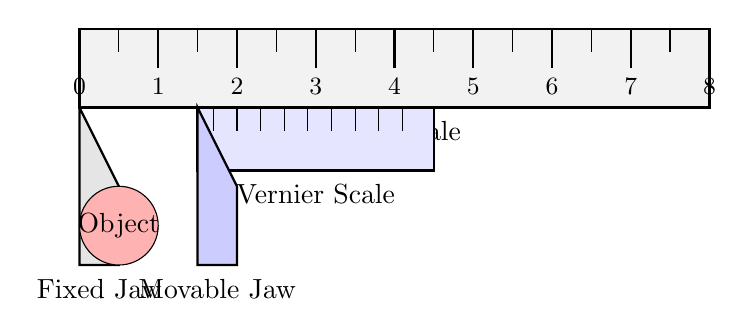
\begin{tikzpicture}
    % Main Scale
    \draw[thick, fill=gray!10] (0,0) rectangle (8, 1);
    \foreach \x in {0.5,1,...,7.5} \draw (\x, 1) -- (\x, 0.7);
    \foreach \x in {0,1,...,8} \draw[thick] (\x, 1) -- (\x, 0.5) node[below] {\small \x};
    \node at (4, -0.3) {Main Scale};
    
    % Vernier Scale
    \draw[thick, fill=blue!10] (1.5, 0) rectangle (4.5, -0.8);
    \foreach \x in {1.7,2.0,...,4.3} \draw (\x, 0) -- (\x, -0.3);
    \node at (3, -1.1) {Vernier Scale};
    
    % Jaws
    \draw[thick, fill=gray!20] (0,0) -- (0,-2) -- (0.5,-2) -- (0.5,-1) -- cycle; % Fixed Jaw
    \node at (0.25, -2.3) {Fixed Jaw};
    
    \draw[thick, fill=blue!20] (1.5,0) -- (1.5,-2) -- (2,-2) -- (2,-1) -- cycle; % Movable Jaw
    \node at (1.75, -2.3) {Movable Jaw};
    
    % Object
    \draw[fill=red!30] (0.5, -1.5) circle (0.5);
    \node at (0.5, -1.5) {Object};
\end{tikzpicture}
\captionof{figure}{Vernier Caliper Construction}
\end{center}

\begin{itemize}
    \item \textbf{Main scale}: Fixed scale with millimeter divisions
    \item \textbf{Vernier scale}: Sliding scale with divisions slightly smaller than main scale
    \item \textbf{Fixed jaw}: Connected to main scale
    \item \textbf{Movable jaw}: Attached to vernier scale
    \item \textbf{Depth rod}: For measuring depths
    \item \textbf{Locking screw}: To fix position during measurement
\end{itemize}

\textbf{Working}: Object is placed between jaws, movable jaw is adjusted to hold object firmly. Reading is taken by noting main scale reading and adding vernier coincidence value.

\textbf{Least Count}: Smallest measurement possible with vernier caliper.
\[ \text{LC} = \frac{1 \text{ division on main scale}}{\text{Number of divisions on vernier scale}} \]

\textbf{Zero Error}: Error when caliper shows non-zero reading with jaws closed.
\begin{itemize}
    \item \textbf{Positive error}: Subtract from reading
    \item \textbf{Negative error}: Add to reading
\end{itemize}
\end{solutionbox}

\begin{mnemonicbox}
\mnemonic{"Very Careful Measurements Leave Count Errors Zero"}
\end{mnemonicbox}

\questionmarks{1(c)(i)}{4}{Distinguish between accuracy and precision.}

\begin{solutionbox}
\begin{answertable}{Accuracy vs Precision}
\begin{tabulary}{\linewidth}{|L|L|}
\hline
\textbf{Accuracy} & \textbf{Precision} \\ \hline
Closeness of measurement to true value & Repeatability of measurement \\ \hline
Affected by systematic errors & Affected by random errors \\ \hline
Represented by mean of measurements & Represented by standard deviation \\ \hline
Improved by calibration & Improved by using better instruments \\ \hline
Example: If true value is 10 cm, measurements of 9.9, 10.1, and 10.0 cm are accurate & Example: Measurements of 9.8, 9.8, 9.8 cm are precise but not accurate if true value is 10 cm \\ \hline
\end{tabulary}
\end{answertable}
\end{solutionbox}

\begin{mnemonicbox}
\mnemonic{"Accurate measurements Are Always At true value, Precise measurements Produce Perfect repeatability"}
\end{mnemonicbox}

\questionmarks{1(c)(ii)}{2}{Pitch of a micrometer screw gauge is 0.5 mm and there are 50 divisions on its circular scale. Find its least count.}

\begin{solutionbox}
\textbf{Formula}: 
\[ \text{Least Count} = \frac{\text{Pitch}}{\text{Number of divisions on circular scale}} \]

\textbf{Calculation}:
\[ \text{LC} = \frac{0.5 \text{ mm}}{50} = 0.01 \text{ mm} \]

\textbf{Least Count of micrometer screw gauge = 0.01 mm}
\end{solutionbox}

\questionmarks{1(c)(iii)}{1}{What is SI unit of heat?}

\begin{solutionbox}
SI unit of heat is \textbf{Joule (J)}
\end{solutionbox}

\orquestionmarks{1(c)(i)}{4}{How are absolute and relative errors calculated?}

\begin{solutionbox}
\textbf{Absolute Error ($\Delta a$)}: Difference between measured value and true value.
For multiple measurements, it's difference between measured value and mean value.

\textbf{Calculation of Absolute Error}:
\begin{itemize}
    \item \textbf{Single measurement}: $\Delta a = |\text{Measured value} - \text{True value}|$
    \item \textbf{Multiple measurements}: 
    \begin{enumerate}
        \item Calculate mean ($a_m$)
        \item For each measurement: $\Delta a_i = |a_i - a_m|$
        \item Mean absolute error: $\Delta a = (\Delta a_1 + \Delta a_2 + ... + \Delta a_n) \div n$
    \end{enumerate}
\end{itemize}

\textbf{Relative Error ($\epsilon_r$)}: Ratio of absolute error to true value.
\[ \epsilon_r = \frac{\text{Absolute error}}{\text{True value}} = \frac{\Delta a}{\text{True value}} \]

\textbf{Percentage Error ($\epsilon_p$)}: Relative error expressed as percentage.
\[ \epsilon_p = \text{Relative error} \times 100 = \left(\frac{\Delta a}{\text{True value}}\right) \times 100\% \]
\end{solutionbox}

\begin{mnemonicbox}
\mnemonic{"Absolute Always measures Actual deviation; Relative References the total value"}
\end{mnemonicbox}

\orquestionmarks{1(c)(ii)}{2}{Main scale of a vernier caliper is calibrated in mm and there are 50 divisions on its vernier scale. Find its least count.}

\begin{solutionbox}
\textbf{Formula}: 
\[ \text{Least Count} = \frac{1 \text{ division on main scale}}{\text{Number of divisions on vernier scale}} \]

\textbf{Calculation}:
1 division on main scale = 1 mm
\[ \text{LC} = \frac{1 \text{ mm}}{50} = 0.02 \text{ mm} \]

\textbf{Least Count of vernier caliper = 0.02 mm}
\end{solutionbox}

\orquestionmarks{1(c)(iii)}{1}{In which of the mode of heat transfer, medium is not required?}

\begin{solutionbox}
\textbf{Radiation} does not require a medium for heat transfer.
\end{solutionbox}

\questionmarks{2(a)}{3}{Write characteristics of electric field lines.}

\begin{solutionbox}
\textbf{Characteristics of Electric Field Lines}:
\begin{enumerate}
    \item Electric field lines start from positive charge and end on negative charge
    \item Field lines never cross each other
    \item Field lines are always perpendicular to the surface of conductor
    \item Number of field lines is proportional to magnitude of charge
    \item Closer field lines indicate stronger electric field
    \item Field lines are continuous curves
    \item Field lines contract longitudinally and expand laterally
\end{enumerate}

\begin{answerdiagram}{Electric Field Lines Geometry}
\begin{tikzpicture}
    % Positive charge
    \node[circle, draw, fill=blue!10, minimum size=0.8cm] (P) at (-2,0) {+};
    % Negative charge
    \node[circle, draw, fill=red!10, minimum size=0.8cm] (N) at (2,0) {-};
    
    % Field lines
    \foreach \angle in {0, 45, ..., 315} {
        \draw[->, Blue] (P) -- +(\angle:0.8cm);
    }
    \foreach \angle in {0, 45, ..., 315} {
        \draw[<-, Red] (N) -- +(\angle:0.8cm);
    }
    
    % Connecting lines
    \draw[->, thick, purple, bending] (P) to[out=45,in=135] (N);
    \draw[->, thick, purple, bending] (P) to[out=-45,in=-135] (N);
    \draw[->, thick, purple] (P) -- (N);
    
    % Non-crossing annotation
    \node at (0, -1.5) {\small Lines start at + and end at -};
\end{tikzpicture}
\end{answerdiagram}
\end{solutionbox}

\begin{mnemonicbox}
\mnemonic{"Electric Field Lines: Start Positive, End Negative, Cross Never"}
\end{mnemonicbox}

\questionmarks{2(b)}{4}{Explain Coulomb's inverse square law for electrostatic forces.}

\begin{solutionbox}
\textbf{Coulomb's Inverse Square Law}: The electrostatic force between two point charges is directly proportional to the product of magnitudes of charges and inversely proportional to the square of distance between them.

\textbf{Mathematical Form}:
\[ F = k \frac{q_1 q_2}{r^2} \]

Where:
\begin{itemize}
    \item $F$ = electrostatic force (in Newtons)
    \item $k$ = electrostatic constant ($9\times 10^9$ N·m$^2$/C$^2$)
    \item $q_1, q_2$ = magnitudes of charges (in Coulombs)
    \item $r$ = distance between charges (in meters)
\end{itemize}

\textbf{Properties}:
\begin{itemize}
    \item \textbf{Vector Quantity}: Force acts along the line joining the two charges
    \item \textbf{Attractive/Repulsive}: Like charges repel, unlike charges attract
    \item \textbf{Central Force}: Follows Newton's third law
    \item \textbf{Medium Dependence}: Depends on the medium between charges ($k$ changes)
\end{itemize}

\begin{answerdiagram}{Coulomb's Law Interation}
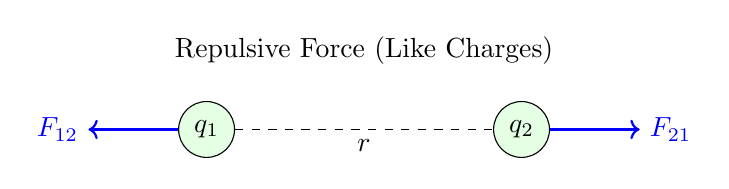
\begin{tikzpicture}
    \node[circle, draw, fill=green!10] (q1) at (0,0) {$q_1$};
    \node[circle, draw, fill=green!10] (q2) at (4,0) {$q_2$};
    
    \draw[dashed] (q1) -- (q2) node[midway, below] {$r$};
    
    \draw[->, thick, blue] (q1) -- (-1.5,0) node[left] {$F_{12}$};
    \draw[->, thick, blue] (q2) -- (5.5,0) node[right] {$F_{21}$};
    
    \node at (2, 1) {Repulsive Force (Like Charges)};
\end{tikzpicture}
\end{answerdiagram}
\end{solutionbox}

\begin{mnemonicbox}
\mnemonic{"Charges Attract/Repel Leveraging Distance Squared"}
\end{mnemonicbox}

\questionmarks{2(c)(i)}{4}{Derive formula for equivalent capacitance of capacitors connected in series and parallel combination.}

\begin{solutionbox}
\textbf{For Series Combination}:

\begin{answerdiagram}{Capacitors in Series}
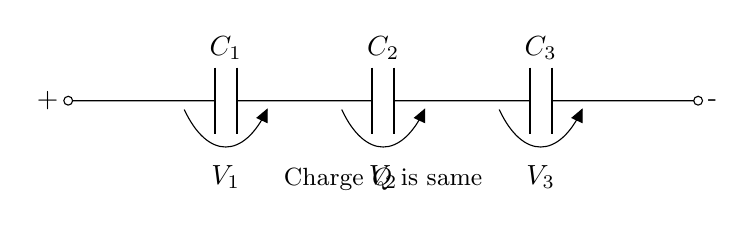
\begin{tikzpicture}
    \draw (0,2) to[short, o-] (1,2)
          to[C, l=$C_1$, v=$V_1$] (3,2)
          to[C, l=$C_2$, v=$V_2$] (5,2)
          to[C, l=$C_3$, v=$V_3$] (7,2)
          to[short, -o] (8,2);
    \node at (0,2) [left] {+};
    \node at (8,2) [right] {-};
    \node at (4,1) {\small Charge $Q$ is same};
\end{tikzpicture}
\end{answerdiagram}

When capacitors are connected in series:
\begin{itemize}
    \item Same charge $Q$ appears on each capacitor
    \item Potential difference distributes across capacitors
    \item $V = V_1 + V_2 + V_3$
\end{itemize}

For each capacitor: $V_1 = Q/C_1$, $V_2 = Q/C_2$, $V_3 = Q/C_3$

Total voltage: 
\[ V = \frac{Q}{C_1} + \frac{Q}{C_2} + \frac{Q}{C_3} = Q \left(\frac{1}{C_1} + \frac{1}{C_2} + \frac{1}{C_3}\right) \]

For equivalent capacitance: $V = Q/C_{eq}$

Therefore: 
\[ \frac{1}{C_{eq}} = \frac{1}{C_1} + \frac{1}{C_2} + \frac{1}{C_3} \]

\textbf{For Parallel Combination}:

\begin{answerdiagram}{Capacitors in Parallel}
\begin{tikzpicture}
    \draw (0,2) to[short, o-] (2,2) -- (2,3) to[C, l=$C_1$] (6,3) -- (6,2) to[short, -o] (8,2);
    \draw (2,2) to[C, l=$C_2$] (6,2);
    \draw (2,2) -- (2,1) to[C, l=$C_3$] (6,1) -- (6,2);
    
    \node at (0,2) [left] {+};
    \node at (8,2) [right] {-};
    \node at (4,-0.5) {\small Voltage $V$ is same};
\end{tikzpicture}
\end{answerdiagram}

When capacitors are connected in parallel:
\begin{itemize}
    \item Same potential difference $V$ across each capacitor
    \item Total charge distributes among capacitors
    \item $Q = Q_1 + Q_2 + Q_3$
\end{itemize}

For each capacitor: $Q_1 = C_1V$, $Q_2 = C_2V$, $Q_3 = C_3V$

Total charge: 
\[ Q = C_1V + C_2V + C_3V = (C_1 + C_2 + C_3)V \]

For equivalent capacitance: $Q = C_{eq}V$

Therefore: 
\[ C_{eq} = C_1 + C_2 + C_3 \]
\end{solutionbox}

\begin{mnemonicbox}
\mnemonic{"Series Sums Reciprocals, Parallel Puts Capacitance Together"}
\end{mnemonicbox}

\questionmarks{2(c)(ii)}{2}{Two capacitors of capacitances 8 $\mu$F and 9 $\mu$F are connected in parallel combination. Find equivalent capacitance.}

\begin{solutionbox}
\textbf{Formula for parallel combination}: $C_{eq} = C_1 + C_2$

\textbf{Given}:
\begin{itemize}
    \item $C_1 = 8 \mu\text{F}$
    \item $C_2 = 9 \mu\text{F}$
\end{itemize}

\textbf{Calculation}:
\[ C_{eq} = 8 \mu\text{F} + 9 \mu\text{F} = 17 \mu\text{F} \]

\textbf{Therefore, equivalent capacitance = 17 $\mu$F}
\end{solutionbox}

\questionmarks{2(c)(iii)}{1}{Write full name of "LASER".}

\begin{solutionbox}
\textbf{LASER}: Light Amplification by Stimulated Emission of Radiation
\end{solutionbox}

\orquestionmarks{2(a)}{3}{What is a capacitor? Define capacitance and write its unit.}

\begin{solutionbox}
\textbf{Capacitor}: A device that stores electric charge and electrical energy in the form of electric field.

\textbf{Capacitance}: The ability of a capacitor to store electric charge. It is defined as the ratio of charge stored to the potential difference applied.

\textbf{Mathematical Form}:
\[ C = \frac{Q}{V} \]

Where:
\begin{itemize}
    \item $C$ = capacitance
    \item $Q$ = charge stored on capacitor
    \item $V$ = potential difference across capacitor
\end{itemize}

\textbf{Unit of Capacitance}: Farad (F)

\begin{answerdiagram}{Parallel Plate Capacitor}
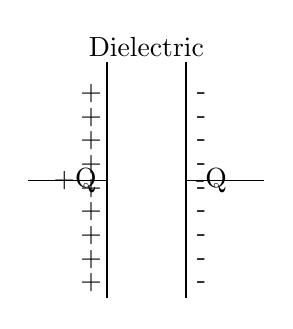
\begin{tikzpicture}
    \draw[thick] (0, 0) -- (0, 3) node[midway, left] {+Q}; 
    \draw[thick] (1, 0) -- (1, 3) node[midway, right] {-Q};
    \draw (0, 1.5) -- (-1, 1.5);
    \draw (1, 1.5) -- (2, 1.5);
    \foreach \y in {0.2, 0.5, ..., 2.8} \node at (-0.2, \y) {+};
    \foreach \y in {0.2, 0.5, ..., 2.8} \node at (1.2, \y) {-};
    \node at (0.5, 3.2) {Dielectric};
\end{tikzpicture}
\end{answerdiagram}
\end{solutionbox}

\begin{mnemonicbox}
\mnemonic{"Capacitors Collect Charge, Volts Vary Fastidiously"}
\end{mnemonicbox}

\orquestionmarks{2(b)}{4}{Explain intensity of electric field and electric potential.}

\begin{solutionbox}
\textbf{Electric Field Intensity}:
\begin{itemize}
    \item \textbf{Definition}: Force experienced by unit positive charge placed at that point
    \item \textbf{Formula}: $E = F/q$
    \item \textbf{Unit}: Newton/Coulomb (N/C) or Volt/meter (V/m)
    \item \textbf{Vector Quantity}: Has both magnitude and direction
    \item \textbf{Direction}: Same as force on positive charge
\end{itemize}

\textbf{Electric Potential}:
\begin{itemize}
    \item \textbf{Definition}: Work done to bring unit positive charge from infinity to that point
    \item \textbf{Formula}: $V = W/q$
    \item \textbf{Unit}: Volt (V) or Joule/Coulomb (J/C)
    \item \textbf{Scalar Quantity}: Has only magnitude
    \item \textbf{Relation with field}: $E = -dV/dr$ (field is negative gradient of potential)
\end{itemize}

\begin{answertable}{Field vs Potential}
\begin{tabulary}{\linewidth}{|L|L|L|}
\hline
\textbf{Property} & \textbf{Electric Field} & \textbf{Electric Potential} \\ \hline
Definition & Force per unit charge & Work done per unit charge \\ \hline
Nature & Vector & Scalar \\ \hline
Unit & N/C or V/m & V or J/C \\ \hline
Dependence & Varies as $1/r^2$ & Varies as $1/r$ \\ \hline
Direction & Away from +ve charge & No direction \\ \hline
\end{tabulary}
\end{answertable}
\end{solutionbox}

\begin{mnemonicbox}
\mnemonic{"Electric Field Forces charges; Potential Provides energy"}
\end{mnemonicbox}

\orquestionmarks{2(c)(i)}{4}{Using formula of capacitance of a parallel plate capacitor, explain effect of plate area, separation between plates and presence of dielectric material between the plates on its capacitance.}

\begin{solutionbox}
\textbf{Formula for capacitance of parallel plate capacitor}:
\[ C = \frac{\epsilon_0 \epsilon_r A}{d} \]

Where:
\begin{itemize}
    \item $C$ = capacitance
    \item $\epsilon_0$ = permittivity of free space ($8.85\times 10^{-12}$ F/m)
    \item $\epsilon_r$ = relative permittivity of dielectric
    \item $A$ = area of overlap between plates
    \item $d$ = distance between plates
\end{itemize}

\textbf{Effect of Plate Area ($A$)}:
\begin{itemize}
    \item Capacitance is directly proportional to area of plates
    \item Increasing area $\rightarrow$ Increases capacitance
    \item Doubling area $\rightarrow$ Doubles capacitance
\end{itemize}

\textbf{Effect of Separation ($d$)}:
\begin{itemize}
    \item Capacitance is inversely proportional to distance between plates
    \item Increasing separation $\rightarrow$ Decreases capacitance
    \item Doubling separation $\rightarrow$ Halves capacitance
\end{itemize}

\textbf{Effect of Dielectric Material ($\epsilon_r$)}:
\begin{itemize}
    \item Capacitance is directly proportional to relative permittivity of dielectric
    \item Inserting dielectric $\rightarrow$ Increases capacitance
    \item Dielectric constant measures this increase: $C_{\text{dielectric}} = \epsilon_r \times C_{\text{air}}$
\end{itemize}

\begin{answerdiagram}{Factors Affecting Capacitance}
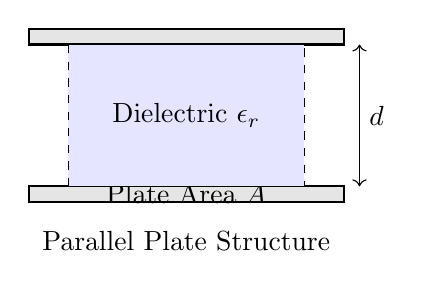
\begin{tikzpicture}
    % Plates
    \draw[thick, fill=gray!20] (0,0) rectangle (4,0.2) node[midway] {Plate Area $A$};
    \draw[thick, fill=gray!20] (0,2) rectangle (4,2.2);
    
    % Distance
    \draw[<->] (4.2, 0.2) -- (4.2, 2) node[midway, right] {$d$};
    
    % Dielectric
    \draw[fill=blue!10, dashed] (0.5, 0.2) rectangle (3.5, 2) node[midway] {Dielectric $\epsilon_r$};
    
    \node at (2, -0.5) {Parallel Plate Structure};
\end{tikzpicture}
\end{answerdiagram}
\end{solutionbox}

\begin{mnemonicbox}
\mnemonic{"Area Amplifies, Distance Diminishes, Dielectrics Double"}
\end{mnemonicbox}

\orquestionmarks{2(c)(ii)}{2}{Voltage between plates of a capacitor of capacitance 0.5 $\mu$F is 150 V. Find magnitude of electric charge on plates.}

\begin{solutionbox}
\textbf{Formula}: $Q = CV$

\textbf{Given}:
\begin{itemize}
    \item Capacitance ($C$) = 0.5 $\mu$F = $0.5 \times 10^{-6}$ F
    \item Voltage ($V$) = 150 V
\end{itemize}

\textbf{Calculation}:
\[ Q = CV = 0.5 \times 10^{-6} \times 150 = 75 \times 10^{-6} \text{ C} = 75 \mu\text{C} \]

\textbf{Therefore, charge on plates = 75 $\mu$C}
\end{solutionbox}

\orquestionmarks{2(c)(iii)}{1}{Of the two parts of an optical fiber, the core and the cladding, which one has larger refractive index?}

\begin{solutionbox}
The \textbf{core} has a larger refractive index than the cladding.
\end{solutionbox}

\questionmarks{3(a)}{3}{Define conduction and convection of heat.}

\begin{solutionbox}
\textbf{Heat Conduction}:
\begin{itemize}
    \item Transfer of heat through matter without actual movement of particles
    \item Occurs due to direct molecular collisions
    \item Heat flows from higher to lower temperature region
    \item Metals are good conductors of heat
    \item Examples: Heat transfer through metal rod, cooking pot
\end{itemize}

\textbf{Heat Convection}:
\begin{itemize}
    \item Transfer of heat through actual movement of matter
    \item Occurs in fluids (liquids and gases)
    \item Involves formation of convection currents
    \item Examples: Room heater, sea breeze, boiling water
\end{itemize}

\begin{answerdiagram}{Modes of Heat Transfer}
\begin{tikzpicture}
    % Conduction
    \node[gtu block] (hot) at (0,0) {Hot};
    \node[gtu block] (cold) at (4,0) {Cold};
    \draw[->, thick, red, snake=snake] (hot) -- (cold) node[midway, above] {Conduction (Solid)};
    
    % Convection
    \draw[fill=blue!10] (6,-1) rectangle (8,1);
    \node at (7, -1.3) {Fluid};
    \draw[->, thick, red, bend right] (6.5, -0.5) to (7.5, 0.5);
    \draw[->, thick, blue, bend right] (7.5, 0.5) to (6.5, -0.5);
    \node at (7, 1.2) {Convection Currents};
\end{tikzpicture}
\end{answerdiagram}
\end{solutionbox}

\begin{mnemonicbox}
\mnemonic{"Conduction Connects molecules; Convection Carries material"}
\end{mnemonicbox}

\questionmarks{3(b)}{4}{Explain construction and working of mercury thermometer.}

\begin{solutionbox}
\textbf{Construction of Mercury Thermometer}:

\begin{answerdiagram}{Mercury Thermometer}
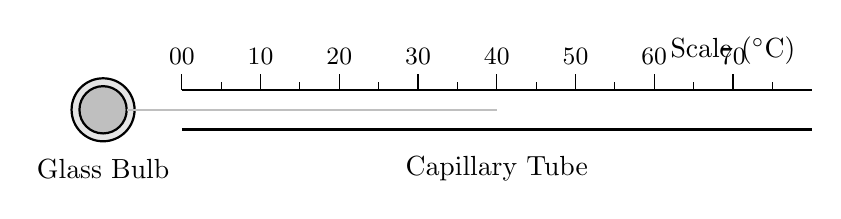
\begin{tikzpicture}
    \draw[thick] (0,0) -- (8,0);
    \draw[thick] (0,0.5) -- (8,0.5);
    \draw[thick, fill=gray!20] (-1, 0.25) circle (0.4); % Bulb
    \draw[thick, fill=gray!50] (-1, 0.25) circle (0.3); % Mercury
    \draw[thick, gray!50] (-0.7, 0.25) -- (4, 0.25); % Mercury thread
    
    % Scale
    \foreach \x in {0,1,...,7} \draw (\x, 0.5) -- (\x, 0.7) node[above] {\small \x0};
    \foreach \x in {0.5,1.5,...,7.5} \draw (\x, 0.5) -- (\x, 0.6);
    
    \node at (-1, -0.5) {Glass Bulb};
    \node at (4, -0.5) {Capillary Tube};
    \node at (7, 1.0) {Scale ($^{\circ}$C)};
\end{tikzpicture}
\end{answerdiagram}

\begin{itemize}
    \item \textbf{Glass bulb}: Contains mercury, acts as reservoir
    \item \textbf{Capillary tube}: Thin glass tube connected to bulb
    \item \textbf{Scale}: Calibrated with temperature markings
    \item \textbf{Protective glass cover}: Protects capillary tube and scale
\end{itemize}

\textbf{Working Principle}:
\begin{enumerate}
    \item Based on thermal expansion of mercury
    \item When temperature increases, mercury expands and rises in capillary
    \item When temperature decreases, mercury contracts and level falls
    \item Temperature is read from scale at mercury level
\end{enumerate}

\textbf{Temperature Range}: -38.83$^{\circ}$C to 356.73$^{\circ}$C.

\textbf{Advantages}: High accuracy, Linear expansion, Visible.
\textbf{Limitations}: Toxic mercury, Cannot measure very low temps.
\end{solutionbox}

\begin{mnemonicbox}
\mnemonic{"Mercury Moves Through Capillary, Showing Temperature"}
\end{mnemonicbox}

\questionmarks{3(c)(i)}{4}{State laws of thermal conductivity and derive formula of coefficient of thermal conductivity.}

\begin{solutionbox}
\textbf{Laws of Thermal Conductivity}:
\begin{enumerate}
    \item Heat flow is directly proportional to temperature difference ($\Delta T$)
    \item Heat flow is directly proportional to cross-sectional area ($A$)
    \item Heat flow is inversely proportional to length ($L$)
    \item Heat flow is directly proportional to time ($t$)
\end{enumerate}

\textbf{Derivation of Coefficient of Thermal Conductivity}:

According to Fourier's law:
\[ Q \propto A \times t \times \frac{\Delta T}{L} \]

Converting to equation with proportionality constant $K$:
\[ Q = K \times A \times t \times \frac{\Delta T}{L} \]

Rearranging:
\[ K = \frac{Q \times L}{A \times t \times \Delta T} \]

Where:
\begin{itemize}
    \item $Q$ = Heat conducted (in Joules)
    \item $L$ = Length of conductor (in meters)
    \item $A$ = Cross-sectional area (in m$^2$)
    \item $t$ = Time (in seconds)
    \item $\Delta T$ = Temperature difference (in Kelvin)
    \item $K$ = Coefficient of thermal conductivity (in W/m·K)
\end{itemize}

\begin{answerdiagram}{Thermal Conduction Model}
\begin{tikzpicture}
    % Bar
    \draw[thick, fill=orange!10] (0,0) rectangle (4,1);
    \node at (2, 0.5) {Conductor (Length $L$, Area $A$)};
    
    % Temps
    \node at (-1, 0.5) {Hot $T_1$};
    \node at (5, 0.5) {Cold $T_2$};
    
    % Heat flow
    \draw[->, UltraThick, red] (-0.5, 0.5) -- (0, 0.5);
    \draw[->, UltraThick, red] (4, 0.5) -- (4.5, 0.5) node[right] {Heat $Q$};
\end{tikzpicture}
\end{answerdiagram}
\end{solutionbox}

\begin{mnemonicbox}
\mnemonic{"Heat Transfers Faster when Area Larger, Temperature higher, Length shorter"}
\end{mnemonicbox}

\questionmarks{3(c)(ii)}{2}{The total area of glass window pane is 0.5 m$^2$. Calculate amount of heat conducted per hour through the pane if thickness of glass is 0.6 cm, the inside temperature is 30$^{\circ}$C and outside temperature is 20$^{\circ}$C. Coefficient of thermal conductivity of glass is 1.0 Wm$^{-1}$K$^{-1}$.}

\begin{solutionbox}
\textbf{Formula}: $Q = \frac{K \times A \times t \times \Delta T}{L}$

\textbf{Given}:
\begin{itemize}
    \item Area ($A$) = 0.5 m$^2$
    \item Thickness ($L$) = 0.6 cm = 0.006 m
    \item Inside temperature ($T_1$) = 30$^{\circ}$C
    \item Outside temperature ($T_2$) = 20$^{\circ}$C
    \item Temperature difference ($\Delta T$) = 10$^{\circ}$C = 10 K
    \item Coefficient of thermal conductivity ($K$) = 1.0 W/m·K
    \item Time ($t$) = 1 hour = 3600 seconds
\end{itemize}

\textbf{Calculation}:
\[ Q = \frac{1.0 \times 0.5 \times 3600 \times 10}{0.006} \]
\[ Q = \frac{18000}{0.006} \]
\[ Q = 3,000,000 \text{ J} = 3000 \text{ kJ} \]

\textbf{Therefore, heat conducted = 3000 kJ per hour}
\end{solutionbox}

\questionmarks{3(c)(iii)}{1}{Which property of light is responsible for transmission of light through optical fibre?}

\begin{solutionbox}
\textbf{Total Internal Reflection (TIR)} is responsible for transmission of light through optical fiber.
\end{solutionbox}

\orquestionmarks{3(a)}{3}{Define heat capacity and specific heat.}

\begin{solutionbox}
\textbf{Heat Capacity}:
\begin{itemize}
    \item Amount of heat energy required to raise temperature of an object by 1$^{\circ}$C or 1K
    \item Depends on mass and material of object
    \item Formula: $C = Q/\Delta T$
    \item Unit: Joule/Kelvin (J/K)
\end{itemize}

\textbf{Specific Heat}:
\begin{itemize}
    \item Amount of heat energy required to raise temperature of 1 kg of substance by 1$^{\circ}$C or 1K
    \item Property of material, independent of mass
    \item Formula: $c = Q/(m\times\Delta T)$
    \item Unit: Joule/kg·K (J/kg·K)
\end{itemize}

\textbf{Relation}: Heat capacity ($C$) = mass ($m$) $\times$ specific heat ($c$)

\begin{answertable}{Heat Capacity vs Specific Heat}
\begin{tabulary}{\linewidth}{|L|L|L|}
\hline
\textbf{Property} & \textbf{Heat Capacity} & \textbf{Specific Heat} \\ \hline
Definition & Heat per degree for object & Heat per degree per unit mass \\ \hline
Symbol & $C$ & $c$ \\ \hline
Unit & J/K & J/kg·K \\ \hline
Depends on & Mass and material & Only material \\ \hline
Formula & $Q/\Delta T$ & $Q/(m\times\Delta T)$ \\ \hline
\end{tabulary}
\end{answertable}
\end{solutionbox}

\begin{mnemonicbox}
\mnemonic{"Heat Capacity for Complete object, Specific heat for Single kilogram"}
\end{mnemonicbox}

\orquestionmarks{3(b)}{4}{Explain construction and working of optical pyrometer.}

\begin{solutionbox}
\textbf{Construction of Optical Pyrometer}:

\begin{answerdiagram}{Optical Pyrometer Block Diagram}
\begin{tikzpicture}[node distance=1.5cm]
    \node[gtu block] (obj) {Hot Object};
    \node[gtu block, right=of obj] (lens) {Objective Lens};
    \node[gtu block, right=of lens] (lamp) {Filament Lamp};
    \node[gtu block, right=of lamp] (filter) {Red Filter};
    \node[gtu block, right=of filter] (eye) {Eyepiece};
    
    \node[gtu block, below=of lamp] (ammeter) {Ammeter};
    \node[gtu block, left=of ammeter] (bat) {Battery};
    \node[gtu block, right=of ammeter] (rheo) {Rheostat};
    
    \draw[gtu arrow, dashed] (obj) -- (lens);
    \draw[gtu arrow, dashed] (lens) -- (lamp);
    \draw[gtu arrow, dashed] (lamp) -- (filter);
    \draw[gtu arrow, dashed] (filter) -- (eye);
    
    \draw[thick] (bat) -- (ammeter);
    \draw[thick] (ammeter) -- (rheo);
    \draw[thick] (rheo) -| (lamp);
    \draw[thick] (lamp) -| (bat);
\end{tikzpicture}
\end{answerdiagram}

\begin{itemize}
    \item \textbf{Telescope}: To view hot object
    \item \textbf{Filament lamp}: Calibrated tungsten filament
    \item \textbf{Rheostat}: To adjust current through filament
    \item \textbf{Ammeter}: To measure current
    \item \textbf{Red filter}: To match wavelengths
    \item \textbf{Eyepiece}: For viewing
\end{itemize}

\textbf{Working Principle}:
\begin{enumerate}
    \item Based on comparing brightness of hot object with standard lamp filament
    \item Object is viewed through telescope
    \item Current adjusted until filament brightness matches object brightness
    \item At match point, filament "disappears" against object background
    \item Temperature determined from calibrated scale or ammeter reading
\end{enumerate}

\textbf{Temperature Range}: 700$^{\circ}$C to 3000$^{\circ}$C
\end{solutionbox}

\begin{mnemonicbox}
\mnemonic{"Pyrometer Produces Perfect Temperature by Brightness Comparison"}
\end{mnemonicbox}

\orquestionmarks{3(c)(i)}{4}{Define linear thermal expansion of solids and derive formula of coefficient linear thermal expansion.}

\begin{solutionbox}
\textbf{Linear Thermal Expansion}: Increase in length of a solid material when its temperature increases.

\textbf{Coefficient of Linear Thermal Expansion ($\alpha$)}: Fractional change in length per unit change in temperature.

\textbf{Derivation}:
For small temperature changes:
\begin{itemize}
    \item Change in length ($\Delta L$) is directly proportional to original length ($L_0$)
    \item $\Delta L$ is directly proportional to change in temperature ($\Delta T$)
\end{itemize}

Therefore: $\Delta L \propto L_0 \times \Delta T$

Converting to equation with proportionality constant $\alpha$:
\[ \Delta L = \alpha \times L_0 \times \Delta T \]

Rearranging:
\[ \alpha = \frac{\Delta L}{L_0 \times \Delta T} \]

Where:
\begin{itemize}
    \item $\Delta L$ = Change in length (in meters)
    \item $L_0$ = Original length (in meters)
    \item $\Delta T$ = Change in temperature (in Kelvin or Celsius)
    \item $\alpha$ = Coefficient of linear thermal expansion (per $^{\circ}$C or per K)
\end{itemize}

\textbf{Final length}: $L = L_0(1 + \alpha\Delta T)$

\begin{answerdiagram}{Linear Expansion}
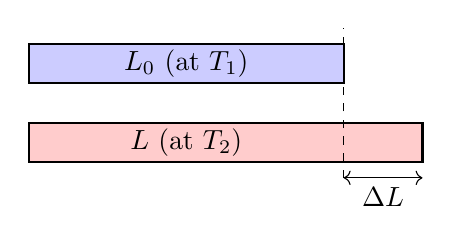
\begin{tikzpicture}
    % Before
    \draw[thick, fill=blue!20] (0,1) rectangle (4,1.5);
    \node at (2, 1.25) {$L_0$ (at $T_1$)};
    
    % After
    \draw[thick, fill=red!20] (0,0) rectangle (5,0.5);
    \draw[dashed] (4, -0.2) -- (4, 1.7);
    \draw[<->] (4, -0.2) -- (5, -0.2) node[midway, below] {$\Delta L$};
    \node at (2, 0.25) {$L$ (at $T_2$)};
\end{tikzpicture}
\end{answerdiagram}
\end{solutionbox}

\begin{mnemonicbox}
\mnemonic{"Linear Expansion Numerically Gives Total Length Increase"}
\end{mnemonicbox}

\orquestionmarks{3(c)(ii)}{2}{Length of a steel rod at 0$^{\circ}$C is 150 cm. What will be its length at 200$^{\circ}$C, if its coefficient of linear thermal expansion is 12 $\times$ 10$^{-6}$ per $^{\circ}$C.}

\begin{solutionbox}
\textbf{Formula}: $L = L_0(1 + \alpha\Delta T)$

\textbf{Given}:
\begin{itemize}
    \item Original length ($L_0$) = 150 cm
    \item Temperature change ($\Delta T$) = 200$^{\circ}$C
    \item Coefficient of linear expansion ($\alpha$) = $12 \times 10^{-6}$ per $^{\circ}$C
\end{itemize}

\textbf{Calculation}:
\[ L = 150(1 + 12 \times 10^{-6} \times 200) \]
\[ L = 150(1 + 24 \times 10^{-4}) \]
\[ L = 150(1 + 0.0024) = 150 \times 1.0024 = 150.36 \text{ cm} \]

\textbf{Therefore, final length of steel rod = 150.36 cm}
\end{solutionbox}

\orquestionmarks{3(c)(iii)}{1}{Which type of emission of radiation is responsible for emission of ordinary light?}

\begin{solutionbox}
\textbf{Spontaneous emission} is responsible for emission of ordinary light.
\end{solutionbox}

\questionmarks{4(a)}{3}{Define amplitude, frequency and time period of a wave.}

\begin{solutionbox}
\textbf{Amplitude}:
\begin{itemize}
    \item Maximum displacement of medium particles from equilibrium position
    \item Represents energy of wave
    \item Denoted by '$A$', measured in meters (m)
\end{itemize}

\textbf{Frequency}:
\begin{itemize}
    \item Number of complete oscillations per unit time
    \item Denoted by '$f$' or '$\nu$', measured in Hertz (Hz)
    \item $f = v/\lambda$
\end{itemize}

\textbf{Time Period}:
\begin{itemize}
    \item Time taken to complete one oscillation
    \item Denoted by '$T$', measured in seconds (s)
    \item $T = 1/f$
\end{itemize}

\begin{answerdiagram}{Wave Parameters}
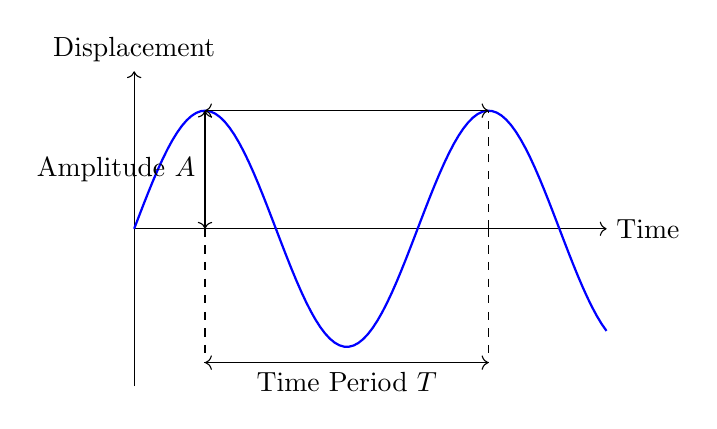
\begin{tikzpicture}
    \draw[->] (0,0) -- (6,0) node[right] {Time};
    \draw[->] (0,-2) -- (0,2) node[above] {Displacement};
    
    \draw[thick, blue, domain=0:6, samples=100] plot (\x, {1.5*sin(100*\x)});
    
    \draw[<->] (0.9,0) -- (0.9,1.5) node[midway, left] {Amplitude $A$};
    \draw[<->] (0.9,1.5) -- (4.5,1.5);
    \draw[dashed] (4.5,0) -- (4.5,1.5);
    
    \draw[<->] (0.9,-1.7) -- (4.5,-1.7) node[midway, below] {Time Period $T$};
    \draw[dashed] (0.9,0) -- (0.9,-1.7);
    \draw[dashed] (4.5,0) -- (4.5,-1.7);
\end{tikzpicture}
\end{answerdiagram}
\end{solutionbox}

\begin{mnemonicbox}
\mnemonic{"Amplitude Adjusts energy, Frequency Finds cycles, Time-period Tracks one cycle"}
\end{mnemonicbox}

\questionmarks{4(b)}{4}{Write difference between transverse and longitudinal waves.}

\begin{solutionbox}
\begin{answertable}{Transverse vs Longitudinal Waves}
\begin{tabulary}{\linewidth}{|L|L|L|}
\hline
\textbf{Property} & \textbf{Transverse Waves} & \textbf{Longitudinal Waves} \\ \hline
Direction of motion & Perpendicular to propagation & Parallel to propagation \\ \hline
Formation of & Crests and troughs & Compressions and rarefactions \\ \hline
Examples & Light, water, EM waves & Sound, seismic P-waves \\ \hline
Medium & Can travel through vacuum & Requires material medium \\ \hline
Polarization & Can be polarized & Cannot be polarized \\ \hline
Equation & $y = A \sin(kx - \omega t)$ & $s = A \sin(kx - \omega t)$ \\ \hline
\end{tabulary}
\end{answertable}

\begin{answerdiagram}{Wave Types}
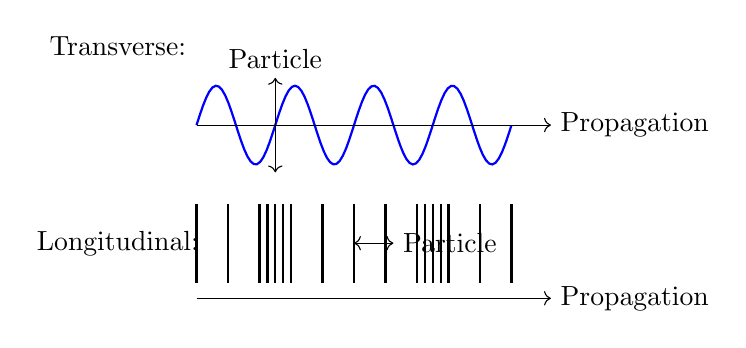
\begin{tikzpicture}
    % Transverse
    \node at (-1, 1) {Transverse:};
    \draw[thick, blue, domain=0:4, samples=100] plot (\x, {0.5*sin(360*\x)});
    \draw[->] (0,0) -- (4.5,0) node[right] {Propagation};
    \draw[<->] (1, -0.6) -- (1, 0.6) node[above] {Particle};
    
    % Longitudinal
    \node at (-1, -1.5) {Longitudinal:};
    \foreach \x in {0, 0.4, 0.8, 1.2, 1.6, 2.0, 2.4, 2.8, 3.2, 3.6, 4.0} {
        \draw[thick] (\x, -1) -- (\x, -2);
    }
    \foreach \x in {0.9, 1.0, 1.1, 2.9, 3.0, 3.1} {
        \draw[thick] (\x, -1) -- (\x, -2); 
    }
    \draw[->] (0,-2.2) -- (4.5,-2.2) node[right] {Propagation};
    \draw[<->] (2, -1.5) -- (2.5, -1.5) node[right] {Particle};
\end{tikzpicture}
\end{answerdiagram}
\end{solutionbox}

\begin{mnemonicbox}
\mnemonic{"Transverse Travels perpendicular, Longitudinal Lies along length"}
\end{mnemonicbox}

\questionmarks{4(c)(i)}{5}{How is ultrasonic wave produced using piezoelectric method?}

\begin{solutionbox}
\begin{answerdiagram}{Piezoelectric Method}
\begin{tikzpicture}[node distance=1.5cm]
    \node[gtu block] (osc) {Oscillator};
    \node[gtu block, right=of osc] (amp) {Amplifier};
    \node[gtu block, right=of amp] (crys) {Piezoelectric Crystal};
    \node[gtu output, right=of crys] (wave) {Ultrasonic Waves};
    
    \draw[gtu arrow] (osc) -- (amp);
    \draw[gtu arrow] (amp) -- (crys);
    \draw[gtu arrow] (crys) -- (wave);
\end{tikzpicture}
\end{answerdiagram}

\textbf{Working Principle}:
\begin{enumerate}
    \item Based on piezoelectric effect.
    \item High-frequency AC voltage applied across piezoelectric crystal (quartz, tourmaline).
    \item Crystal vibrates at frequency of applied voltage.
    \item At resonance (applied frequency = natural frequency), maximum amplitude vibrations occur.
    \item Ultrasonic waves are generated.
\end{enumerate}

\textbf{Frequency Range}: 20 kHz to several MHz.
\textbf{Advantages}: High efficiency, Precise control, Compact.
\end{solutionbox}

\begin{mnemonicbox}
\mnemonic{"Piezo Produces waves when Properly Pulsed with electricity"}
\end{mnemonicbox}

\questionmarks{4(c)(ii)}{2}{Explain any two properties of sound wave.}

\begin{solutionbox}
\begin{enumerate}
    \item \textbf{Reflection of Sound}:
    \begin{itemize}
        \item Bounces back from obstacles
        \item Follows law: angle of incidence = angle of reflection
        \item Creates echoes
    \end{itemize}
    \item \textbf{Refraction of Sound}:
    \begin{itemize}
        \item Bending when passing between media with different speeds
        \item Explains sound focusing and night-time audibility
    \end{itemize}
\end{enumerate}

\begin{answerdiagram}{Sound Properties}
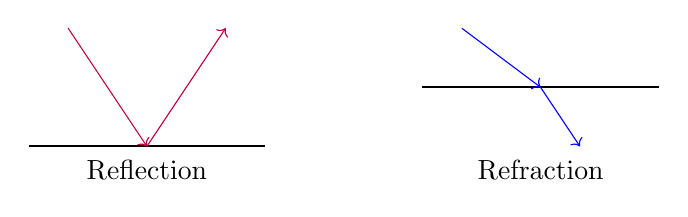
\begin{tikzpicture}
    % Reflection
    \draw[thick] (0,0) -- (3,0);
    \draw[->, purple] (0.5, 1.5) -- (1.5, 0);
    \draw[->, purple] (1.5, 0) -- (2.5, 1.5);
    \node at (1.5, -0.3) {Reflection};
    
    % Refraction
    \draw[thick] (5,0.75) -- (8,0.75);
    \draw[->, blue] (5.5, 1.5) -- (6.5, 0.75);
    \draw[->, blue] (6.5, 0.75) -- (7.0, 0);
    \node at (6.5, -0.3) {Refraction};
\end{tikzpicture}
\end{answerdiagram}
\end{solutionbox}

\begin{mnemonicbox}
\mnemonic{"Sound Shows Remarkable Refractions During travel"}
\end{mnemonicbox}

\orquestionmarks{4(a)}{3}{Define wavelength, phase and velocity of a wave.}

\begin{solutionbox}
\textbf{Wavelength ($\lambda$)}: Distance between two consecutive points in phase. Distance traveled during one complete oscillation. $v = \lambda f$.

\textbf{Phase}: State of oscillation at a specific point and time. Points differing by $2\pi$ are in phase; by $\pi$ are in opposite phase.

\textbf{Velocity ($v$)}: Rate at which wave propagates. $v = \lambda f$. Depends on medium.

\begin{answerdiagram}{Wave Properties}
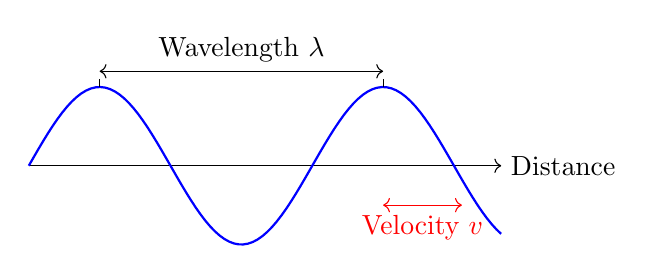
\begin{tikzpicture}
    \draw[->] (0,0) -- (6,0) node[right] {Distance};
    \draw[thick, blue, domain=0:6, samples=100] plot (\x, {sin(100*\x)});
    
    \draw[<->] (0.9, 1.2) -- (4.5, 1.2) node[midway, above] {Wavelength $\lambda$};
    \draw[dashed] (0.9, 1) -- (0.9, 1.2);
    \draw[dashed] (4.5, 1) -- (4.5, 1.2);
    
    \draw[<->, red] (4.5, -0.5) -- (5.5, -0.5) node[midway, below] {Velocity $v$};
\end{tikzpicture}
\end{answerdiagram}
\end{solutionbox}

\begin{mnemonicbox}
\mnemonic{"Wavelength Wraps one cycle, Phase Portrays position, Velocity Values propagation speed"}
\end{mnemonicbox}

\orquestionmarks{4(b)}{4}{Explain constructive and destructive interference of waves.}

\begin{solutionbox}
\textbf{Constructive Interference}:
\begin{itemize}
    \item Waves meet in phase (crest meets crest)
    \item Phase diff = $2n\pi$, Path diff = $n\lambda$
    \item \textbf{Result}: Larger amplitude (sum of individuals)
\end{itemize}

\textbf{Destructive Interference}:
\begin{itemize}
    \item Waves meet in opposite phase (crest meets trough)
    \item Phase diff = $(2n+1)\pi$, Path diff = $(n+1/2)\lambda$
    \item \textbf{Result}: Smaller amplitude (difference of individuals)
\end{itemize}

\begin{answerdiagram}{Interference Types}
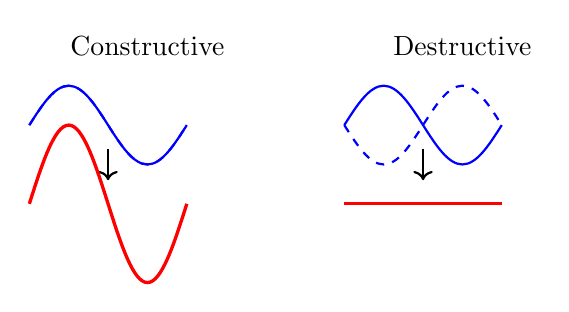
\begin{tikzpicture}
    % Constructive
    \node at (1.5, 2.5) {Constructive};
    \draw[blue, thick] (0,1.5) sin (0.5,2) cos (1,1.5) sin (1.5,1) cos (2,1.5);
    \draw[blue, thick, dashed] (0,1.5) sin (0.5,2) cos (1,1.5) sin (1.5,1) cos (2,1.5);
    \draw[->, thick] (1,1.2) -- (1,0.8);
    \draw[red, very thick] (0,0.5) sin (0.5,1.5) cos (1,0.5) sin (1.5,-0.5) cos (2,0.5);
    
    % Destructive
    \node at (5.5, 2.5) {Destructive};
    \draw[blue, thick] (4,1.5) sin (4.5,2) cos (5,1.5) sin (5.5,1) cos (6,1.5);
    \draw[blue, thick, dashed] (4,1.5) sin (4.5,1) cos (5,1.5) sin (5.5,2) cos (6,1.5);
    \draw[->, thick] (5,1.2) -- (5,0.8);
    \draw[red, very thick] (4,0.5) -- (6,0.5);
\end{tikzpicture}
\end{answerdiagram}
\end{solutionbox}

\begin{mnemonicbox}
\mnemonic{"Constructive Creates Larger waves; Destructive Diminishes wave height"}
\end{mnemonicbox}

\orquestionmarks{4(c)(i)}{5}{How is ultrasonic wave produced using magnetostriction method?}

\begin{solutionbox}
\begin{answerdiagram}{Magnetostriction Oscillator}
\begin{tikzpicture}[node distance=1.5cm]
    \node[gtu block] (osc) {Oscillator};
    \node[gtu block, right=of osc] (amp) {Amplifier};
    \node[gtu block, right=of amp] (coil) {Coil on Ferromagnetic Rod};
    \node[gtu output, right=of coil] (wave) {Ultrasonic Waves};
    
    \draw[gtu arrow] (osc) -- (amp);
    \draw[gtu arrow] (amp) -- (coil);
    \draw[gtu arrow] (coil) -- (wave);
\end{tikzpicture}
\end{answerdiagram}

\textbf{Working Principle}:
\begin{enumerate}
    \item Based on magnetostriction effect (dimensional change in magnetic field).
    \item Alternating magnetic field applied to ferromagnetic rod (Ni, Fe).
    \item Rod expands/contracts at frequency of applied field.
    \item Vibrations generate ultrasonic waves.
\end{enumerate}

\textbf{Frequency Range}: 20 kHz to 100 kHz.
\textbf{Advantages}: High power, Rugged.
\textbf{Limitations}: Low frequency only, Heating issues.
\end{solutionbox}

\begin{mnemonicbox}
\mnemonic{"Magnetic Materials Move Minutely Making ultrasonic waves"}
\end{mnemonicbox}

\orquestionmarks{4(c)(ii)}{2}{Explain any two properties of light wave.}

\begin{solutionbox}
\begin{enumerate}
    \item \textbf{Reflection}: Bouncing back from surface. Angle i = Angle r. Used in mirrors.
    \item \textbf{Refraction}: Bending when changing medium. Snell's law: $n_1 \sin\theta_1 = n_2 \sin\theta_2$. Used in lenses.
\end{enumerate}

\begin{answerdiagram}{Light Properties}
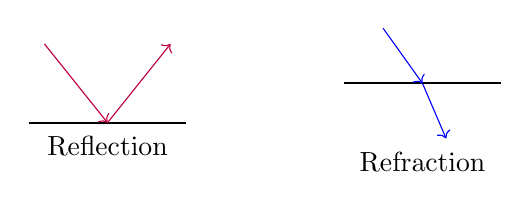
\begin{tikzpicture}
    % Reflection
    \draw[thick] (0,0) -- (2,0);
    \draw[->, purple] (0.2, 1) -- (1, 0);
    \draw[->, purple] (1, 0) -- (1.8, 1);
    \node at (1, -0.3) {Reflection};
    
    % Refraction
    \draw[thick] (4,0.5) -- (6,0.5);
    \draw[->, blue] (4.5, 1.2) -- (5, 0.5);
    \draw[->, blue] (5, 0.5) -- (5.3, -0.2);
    \node at (5, -0.5) {Refraction};
\end{tikzpicture}
\end{answerdiagram}
\end{solutionbox}

\begin{mnemonicbox}
\mnemonic{"Light Likes to Reflect from mirrors and Refract through media"}
\end{mnemonicbox}

\questionmarks{5(a)}{3}{Write characteristics of LASER.}

\begin{solutionbox}
\begin{answertable}{LASER Characteristics}
\begin{tabulary}{\linewidth}{|L|L|}
\hline
\textbf{Characteristic} & \textbf{Description} \\ \hline
Monochromatic & Single wavelength (pure color) \\ \hline
Coherent & Waves in same phase (high interference) \\ \hline
Directional & Minimal divergence over long distance \\ \hline
High Intensity & Concentrated energy \\ \hline
\end{tabulary}
\end{answertable}

\begin{answerdiagram}{Laser vs Ordinary Light}
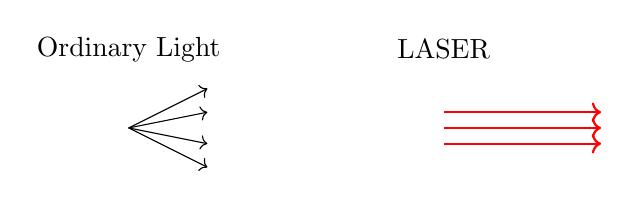
\begin{tikzpicture}
    % Ordinary
    \node at (0, 1) {Ordinary Light};
    \draw[->] (0,0) -- (1,0.5);
    \draw[->] (0,0) -- (1,-0.5);
    \draw[->] (0,0) -- (1,0.2);
    \draw[->] (0,0) -- (1,-0.2);
    
    % Laser
    \node at (4, 1) {LASER};
    \draw[->, thick, red] (4,0.2) -- (6,0.2);
    \draw[->, thick, red] (4,0) -- (6,0);
    \draw[->, thick, red] (4,-0.2) -- (6,-0.2);
\end{tikzpicture}
\end{answerdiagram}
\end{solutionbox}

\begin{mnemonicbox}
\mnemonic{"LASER Light: Monochromatic, Coherent, Directional, Intense"}
\end{mnemonicbox}

\questionmarks{5(b)}{4}{Discuss importance of LASER in engineering and medical field.}

\begin{solutionbox}
\textbf{Engineering}:
\begin{enumerate}
    \item \textbf{Manufacturing}: Cutting, welding, 3D printing.
    \item \textbf{Measurement}: LIDAR, alignment.
    \item \textbf{Communications}: Fiber optics, free-space.
\end{enumerate}

\textbf{Medical}:
\begin{enumerate}
    \item \textbf{Surgery}: Bloodless cutting, LASIK.
    \item \textbf{Diagnostics}: Imaging, spectroscopy.
    \item \textbf{Therapy}: Cancer treatment, pain management.
    \item \textbf{Dentistry}: Teeth whitening.
\end{enumerate}
\end{solutionbox}

\begin{mnemonicbox}
\mnemonic{"LASER Enhances Manufacturing, Measures precisely, Communicates data, Heals patients"}
\end{mnemonicbox}

\questionmarks{5(c)(i)}{5}{What is importance of population inversion and metastable state for production of LASER?}

\begin{solutionbox}
\textbf{Population Inversion}:
\begin{itemize}
    \item State where more atoms are in excited state than ground state.
    \item Essential for stimulated emission to dominate absorption.
    \item Enables light amplification.
\end{itemize}

\textbf{Metastable State}:
\begin{itemize}
    \item Excited state with long lifetime ($10^{-3}$s vs $10^{-8}$s).
    \item Allows accumulation of excited atoms.
    \item Necessary to establish population inversion.
\end{itemize}

\begin{answerdiagram}{Energy Levels}
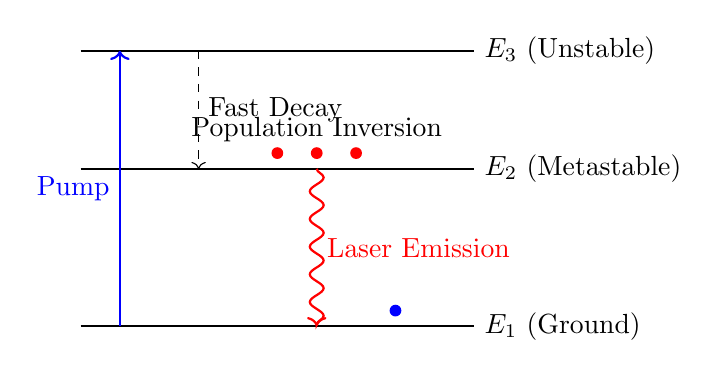
\begin{tikzpicture}
    % Levels
    \draw[thick] (0,0) -- (5,0) node[right] {$E_1$ (Ground)};
    \draw[thick] (0,2) -- (5,2) node[right] {$E_2$ (Metastable)};
    \draw[thick] (0,3.5) -- (5,3.5) node[right] {$E_3$ (Unstable)};
    
    % Pumping
    \draw[->, thick, blue] (0.5,0) -- (0.5,3.5) node[midway, left] {Pump};
    
    % Fast Transition
    \draw[->, dashed] (1.5,3.5) -- (1.5,2) node[midway, right] {Fast Decay};
    
    % Laser
    \draw[->, thick, red, decorate, decoration={snake}] (3,2) -- (3,0) node[midway, right] {Laser Emission};
    
    % Atoms
    \foreach \x in {2.5, 3.0, 3.5} \node[circle, fill=red, inner sep=1.5pt] at (\x, 2.2) {};
    \foreach \x in {4.0} \node[circle, fill=blue, inner sep=1.5pt] at (\x, 0.2) {};
    \node at (3, 2.5) {Population Inversion};
\end{tikzpicture}
\end{answerdiagram}
\end{solutionbox}

\begin{mnemonicbox}
\mnemonic{"Population Inversion Makes Electrons Stay high; Metastable maintains this Situation Longer"}
\end{mnemonicbox}

\questionmarks{5(c)(ii)}{2}{Explain graded index optical fibre.}

\begin{solutionbox}
\textbf{Graded Index (GRIN) Fiber}:
\begin{itemize}
    \item Core refractive index decreases parabolicly from center to periphery ($n(r) = n_1(1 - \alpha r^2)$).
    \item Light travels in curved paths.
    \item Reduces modal dispersion and increases bandwidth.
\end{itemize}

\begin{answerdiagram}{Graded Index Profile}
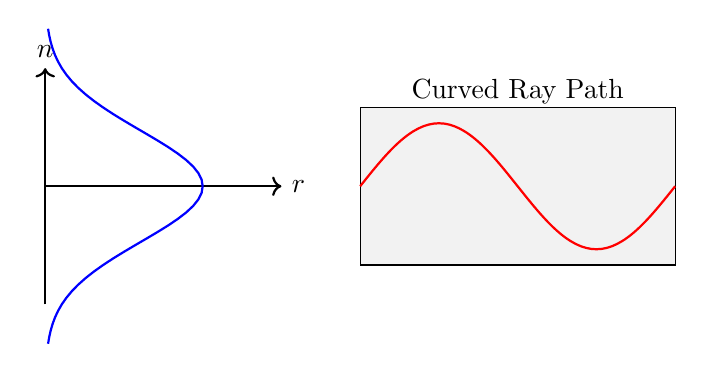
\begin{tikzpicture}
    % Profile
    \draw[thick, ->] (0,-1.5) -- (0,1.5) node[above] {$n$};
    \draw[thick, ->] (0,0) -- (3,0) node[right] {$r$};
    \draw[thick, blue, domain=0:2] plot({2*exp(-\x*\x)}, \x);
    \draw[thick, blue, domain=0:2] plot({2*exp(-\x*\x)}, -\x);
    
    % Ray path
    \draw[fill=gray!10] (4,-1) rectangle (8,1);
    \draw[thick, red] (4,0) sin (5, 0.8) cos (6,0) sin (7,-0.8) cos (8,0);
    \node at (6, 1.2) {Curved Ray Path};
\end{tikzpicture}
\end{answerdiagram}
\end{solutionbox}

\begin{mnemonicbox}
\mnemonic{"Graded Index Gradually Improves transmission by Smoothing dispersion"}
\end{mnemonicbox}

\orquestionmarks{5(a)}{3}{Define refraction of light and write Snell's law.}

\begin{solutionbox}
\textbf{Refraction}: Bending of light passing between media due to speed change.
\textbf{Snell's Law}: Ratio of sines of angles equals ratio of refractive indices.
\[ n_1 \sin \theta_1 = n_2 \sin \theta_2 \]

\begin{answerdiagram}{Refraction}
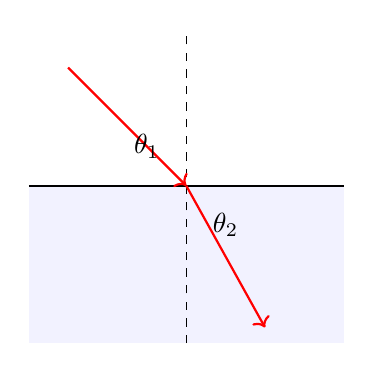
\begin{tikzpicture}
    \fill[blue!5] (0,-2) rectangle (4,0) node[midway] {$n_2$};
    \fill[white] (0,0) rectangle (4,2) node[midway] {$n_1$};
    \draw[thick] (0,0) -- (4,0);
    \draw[dashed] (2,-2) -- (2,2);
    
    \draw[->, red, thick] (0.5, 1.5) -- (2,0);
    \draw[->, red, thick] (2,0) -- (3, -1.8);
    
    \node at (1.5, 0.5) {$\theta_1$};
    \node at (2.5, -0.5) {$\theta_2$};
\end{tikzpicture}
\end{answerdiagram}
\end{solutionbox}

\begin{mnemonicbox}
\mnemonic{"Sine ratios Equal Index ratios"}
\end{mnemonicbox}

\orquestionmarks{5(b)}{4}{Discuss importance of optical fibre in engineering and medical field.}

\begin{solutionbox}
\textbf{Engineering}:
\begin{itemize}
    \item Comms: High speed internet, secure data.
    \item Sensors: Strain, temp monitoring.
    \item Industrial: Remote inspection.
\end{itemize}

\textbf{Medical}:
\begin{itemize}
    \item Diagnostics: Endoscopy.
    \item Surgery: Laser delivery, microsurgery.
    \item Imaging: OCT.
\end{itemize}
\end{solutionbox}

\begin{mnemonicbox}
\mnemonic{"Optical Fibers Connect, Sense, Visualize, and Treat"}
\end{mnemonicbox}

\orquestionmarks{5(c)(i)}{5}{Derive formula for numerical aperture and angle of acceptance of optical fibre.}

\begin{solutionbox}
\textbf{Numerical Aperture (NA)}:
\begin{enumerate}
    \item At core-cladding interface, critical angle $\theta_c$: $\sin \theta_c = n_2/n_1$.
    \item Max angle in core: $90^{\circ} - \theta_c$.
    \item Apply Snell's law at entrance (Air $n_0=1$): $\sin \theta_a = n_1 \sin(90^{\circ} - \theta_c) = n_1 \cos \theta_c$.
    \item Substitute $\cos \theta_c = \sqrt{1 - \sin^2 \theta_c} = \sqrt{1 - (n_2/n_1)^2}$.
    \item $\sin \theta_a = n_1 \sqrt{1 - (n_2/n_1)^2} = \sqrt{n_1^2 - n_2^2}$.
\end{enumerate}

\textbf{Formula}: $\text{NA} = \sin \theta_a = \sqrt{n_1^2 - n_2^2}$

\begin{answerdiagram}{Numerical Aperture}
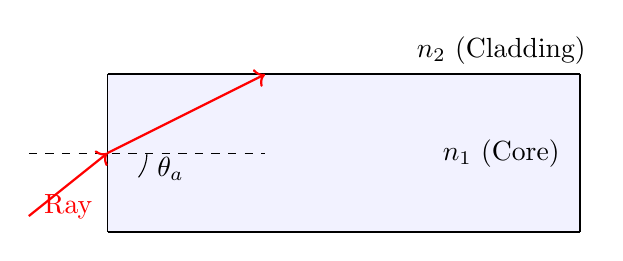
\begin{tikzpicture}
    \draw[thick] (0,0) -- (6,0);
    \draw[thick] (0,2) -- (6,2);
    \draw[fill=blue!5] (0,0) rectangle (6,2);
    \node at (5, 1) {$n_1$ (Core)};
    \node at (5, 2.3) {$n_2$ (Cladding)};
    
    \draw[dashed] (-1, 1) -- (2, 1);
    \draw[->, red, thick] (-1, 0.2) -- (0, 1) node[midway, below] {Ray};
    \draw[->, red, thick] (0, 1) -- (2, 2);
    
    \draw (0.5, 1) arc (0:-38:0.5);
    \node at (0.8, 0.8) {$\theta_a$};
\end{tikzpicture}
\end{answerdiagram}
\end{solutionbox}

\begin{mnemonicbox}
\mnemonic{"NA Notes Acceptance angle; Square root of n-squared difference Shows maximum sine"}
\end{mnemonicbox}

\orquestionmarks{5(c)(ii)}{2}{Explain step index optical fibre.}

\begin{solutionbox}
\textbf{Step Index Fiber}:
\begin{itemize}
    \item Uniform core index $n_1$ surrounded by lower uniform cladding index $n_2$.
    \item Sharp "step" transition.
    \item Types: Single-mode (small core), Multi-mode (large core).
    \item Limitation: Modal dispersion.
\end{itemize}

\begin{answerdiagram}{Step Index Profile}
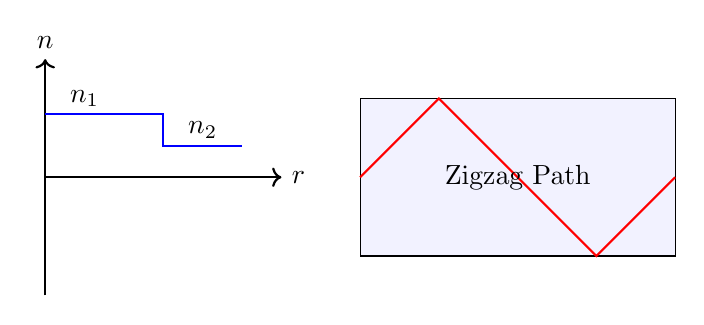
\begin{tikzpicture}
    % Profile
    \draw[thick, ->] (0,0) -- (3,0) node[right] {$r$};
    \draw[thick, ->] (0,-1.5) -- (0,1.5) node[above] {$n$};
    \draw[thick, blue] (0,0.8) -- (1.5,0.8) -- (1.5,0.4) -- (2.5,0.4);
    \node at (0.5, 1) {$n_1$};
    \node at (2, 0.6) {$n_2$};
    
    % Ray
    \draw[fill=blue!5] (4,-1) rectangle (8,1);
    \draw[thick, red] (4,0) -- (5, 1) -- (7, -1) -- (8, 0);
    \node at (6, 0) {Zigzag Path};
\end{tikzpicture}
\end{answerdiagram}
\end{solutionbox}

\begin{mnemonicbox}
\mnemonic{"Step Index Shows Two distinct Indices with Perfect boundary"}
\end{mnemonicbox}

\end{document}

